\documentclass[tikz,border=2mm]{standalone}
\usetikzlibrary{calc,quotes,intersections, angles}

\begin{document}
    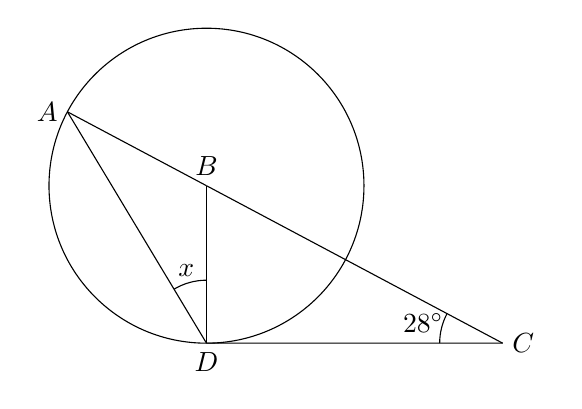
\begin{tikzpicture}[scale=2]
    % mark points on circle
        \coordinate[label = above:$B$] (B) at (0,0);
        \coordinate[label=below:$D$] (D) at (-90:1);

    % draw chords and circle
        \draw[name path=circ] (0,0) circle (1);
        \draw (D) -- (B);
        
    % draw tangent
    \path [name path =Tan1]  (D) -- ($(D)!2!-90:(B)$) coordinate (L);

    %
    \path[name path=BC] (B) -- ($(B)!2.5!62:(D)$);
    \path[name path=DA] (D) -- ($(D)!2!31:(B)$);
    \path[name intersections={of=BC and Tan1, by={C}}];
    \path[name intersections={of=DA and circ, by={A,temp}}];

    \draw (C) -- (B);
    \draw (D) -- (C);
    \draw (D) -- (A);

    % % Label points C and B
    \node at (C) [anchor=west] {$C$};
    \node at (A) [anchor= east] {$A$};

    \draw (A) -- (B);
    % % \draw (A) -- (D);
    
    \pic [draw, "$x$", angle eccentricity=1.2, angle radius = 0.8cm] {angle = B--D--A};
    \pic [draw, "$28^\circ$", angle eccentricity=1.3, angle radius = 0.8cm] {angle = B--C--D};
        
    \end{tikzpicture}
\end{document}